% "{'classe':('PSI'),'chapitre':'stat_mam','type':('td'),'titre':'Machine de forage', 'source':'Concours CCINP 2023 - MP','comp':('B2-14','C1-05','C2-07'),'corrige':False}"
%\setchapterimage{fig_00.jpg}
\chapter*{TD \arabic{cptApplication} \\ 
Machine de forage -- \ifprof Corrigé \else Sujet \fi}
\addcontentsline{toc}{section}{TD \arabic{cptApplication} : Machine de forage -- \ifprof Corrigé \else Sujet \fi}

\iflivret \stepcounter{cptApplication} \else
\ifprof  \stepcounter{cptApplication} \else \fi
\fi

\setcounter{question}{0}
\marginnote{D'après Concours CCINP 2023 -- MP.}
\marginnote[1cm]{
\UPSTIcompetence[2]{B2-14}
\UPSTIcompetence[2]{C1-05}
\UPSTIcompetence[2]{C2-07}
}

\begin{marginfigure}
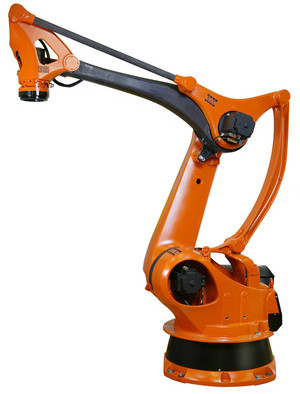
\includegraphics[width=\linewidth]{fig_01}
\end{marginfigure}


Dans le domaine du génie civil, les foreuses permettent de réaliser des perçages profonds afin de couler des pieux en béton armé. On s'intéresse aux conditions de basculement statique de la foreuse. 

Le basculement de la machine peut être dû à un déport trop important du centre de gravité 
de la machine, mais peut aussi être dû à un affaissement du sol. La foreuse doit donc contrôler à tout instant, par estimation, la pression qu’elle exerce sur le sol (et donc que le sol exerce sur elle). 

Le tableau \ref{Cy_11_Ch_01_TD_01_tab_01} récapitule les niveaux de pression que les sols peuvent supporter avant de risquer de s’affaisser. 




\begin{marginfigure}
\centering
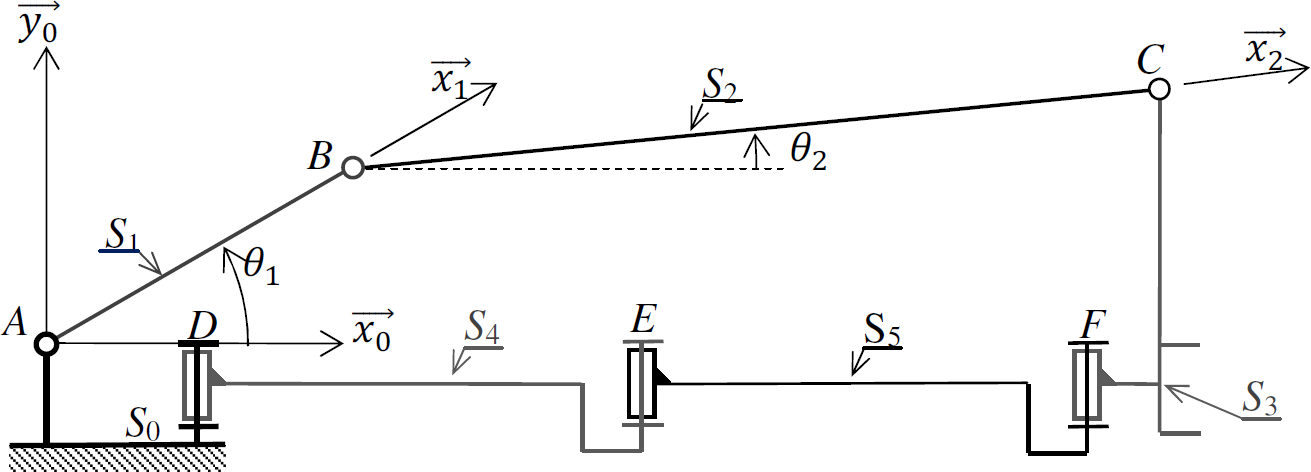
\includegraphics[width=\linewidth]{fig_06}
\caption{Modèles de répartitions trapézoïdales de pression du sol sur les chenilles. \label{Cy_11_Ch_01_TD_01_fig_06}}
\end{marginfigure}

D’après les normes européennes, 
% les  efforts entre le sol et les chenilles ne doivent pas être modélisés comme 
%ponctuels au centre de leur surface de  contact comme cela a été supposé 
%dans la partie précédente (avec $F_d$ et $F_g$). La 
la répartition de pression du sol sur 
chaque chenille doit être modélisée 
comme trapézoïdale sur sa longueur et 
constante sur sa largeur. Un exemple 
de représentations 3D, 2D et << aplatie >> 
%(comme vue sur l’écran de contrôle dans la cabine) 
de telles répartitions est 
donné sur la figure \ref{Cy_11_Ch_01_TD_01_fig_06}. Sur la vue 
<< aplatie >>, la machine est vue de 
dessus et la visualisation de l’allure des 
pressions sous les chenilles est 
ramenée dans le plan.% de l’écran. 

 \begin{table*}
\footnotesize{
\begin{tabular}{p{3cm}ccccccc}
\hline
\textbf{Type de sol} & Rocher & Schiste argileux & Gravier compact & Asphalte & Sable compacté & Sable en 
vrac & Argile humide \\
\textbf{Pression 
maximale 
admissible (kPa)} & 2 000 & 800 & 400&  200&  200&  100 & $<100$ \\ \hline
\end{tabular}}
\caption{Pressions admissibles par le sol selon le type de sol \label{Cy_11_Ch_01_TD_01_tab_01}}
\end{table*}


Un des rôles de l’ordinateur de bord est 
d’estimer ces répartitions de pression 
afin de vérifier que la pression 
maximale supportée par le sol (rentrée 
par l’utilisateur en fonction du site) n’est 
pas atteinte à un coefficient de sécurité 
près. 
Si c’est le cas, l’ordinateur bloque tous 
les mouvements de la foreuse qui 
risqueraient d’empirer et renvoie une 
alarme. 


 
On se propose dans cette sous-partie 
d’étudier cette estimation. 
 
 On base l’étude sur le paramétrage figure \ref{Cy_11_Ch_01_TD_01_fig_07}, avec répartition de 
pression entre le sol et les chenilles. On note : 
\begin{itemize}
\item $P(x,y,0)$, un point courant de contact entre le sol et les chenilles. Attention, $x$ est négatif sur la 
figure ci-dessous. Les grandeurs $\dd x$ et $\dd y$ sont les dimensions du domaine surfacique élémentaire autour du point $P$ entre le sol et les chenilles ; 
\item $p_g(y)= A \dfrac{y}{L}+B$, la pression du sol 0 sur la chenille gauche $cg$ au point $P(x,y,0)$ où $A$ et $B$, homogènes à des pressions, sont inconnues et à déterminer ; 
\item $p_d(y)= C \dfrac{y}{L}+D$, la pression du sol 0 sur la chenille droite $cd$ au point $P(x,y,0)$ où $C$ et $D$, 
homogènes à des pressions, sont inconnues et à déterminer ; 
\item $L = \SI{5,4}{m}$, la longueur et $l = \SI{1}{m}$ la largeur de chaque chenille ; 
\item $a = \SI{2,1}{m}$, la distance moyenne sur l’axe $\vect{x}$ d’une chenille au centre $O$ de la machine. 
\end{itemize}

\begin{marginfigure}
\centering
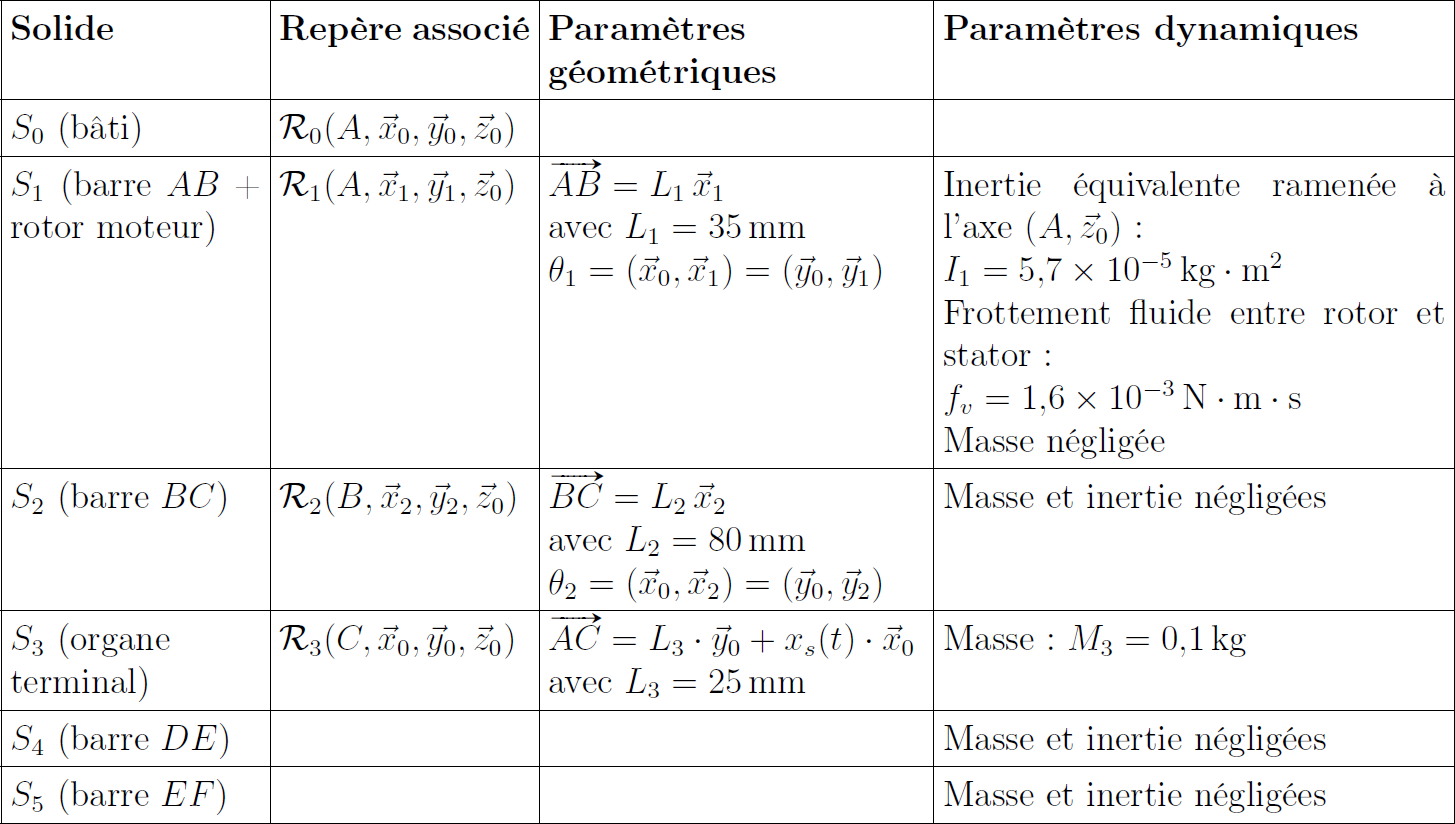
\includegraphics[width=\linewidth]{fig_07}
\caption{Simplification et modèle équivalent  \label{Cy_11_Ch_01_TD_01_fig_07}}
\end{marginfigure}


% \begin{figure}
%\centering
%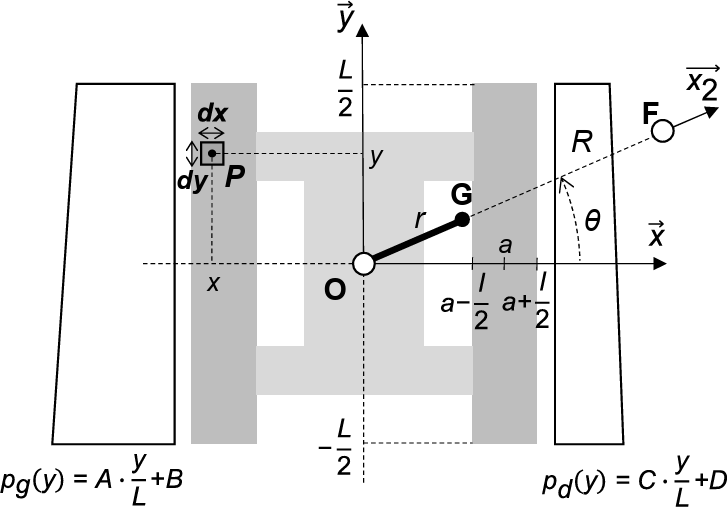
\includegraphics[width=\linewidth]{ann_02}
%%\caption{Simplification et modèle équivalent  \label{Cy_11_Ch_01_TD_01_fig_07}}
%\end{figure}



Afin de résoudre le problème plus 
facilement, on somme les deux 
glisseurs (poids en $G$ et sol en $F$) pour 
en former un seul équivalent (en $E$), 
comme visualisé sur la figure \ref{Cy_11_Ch_01_TD_01_fig_07} et noté 
$\vectf{eq}{f} = \indice{F}{eq} \vect{z}$ où $\indice{F}{eq}$ est négatif. 




\question{Déterminer les expressions de $\indice{F}{eq}$ et de $e$ en fonction de $M$, $m$, $F_w$, $R$, $r$ et de $g$.} 
 
La force élémentaire de réaction du sol 0 sur la chenille gauche $cg$ est notée 
$\vect{\dd F_{0\rightarrow cg}(P)} = p_g(y)\vect{z}\dd x\dd y $. 
La chenille droite est notée $cd$. 
 
\question{En déduire l’expression de la force élémentaire $\vect{\dd F_{0\rightarrow cg}(P)}$  et du moment élémentaire $\vect{\dd M_{O,0\rightarrow cg}(P)}$ 
 au point $O$ qu’exercent le sol sur la chenille gauche en un point $P$ de contact en 
fonction de $A$ et de $B$. }
 
\question{Déterminer à l’aide de la question précédente les expressions de l’effort $\vect{F_{0\rightarrow cg}}$ et du moment au point $O$ $\vect{M_{O,0\rightarrow cg}}$ en fonction de $B$, $D$ et des données connues du système.}
 
 De même, on pourrait, par analogie, déterminer $\vect{F_{0\rightarrow cd}}$ $\vect{M_{O,0\rightarrow cd}}$ en fonction de $C$ et de $D$. Au final, 
on peut en déduire la force $\vect{F_{0\rightarrow \Sigma}}$
 qu’exerce le sol sur la foreuse et le moment en $O$ qu’exerce le sol 
sur la foreuse $\vect{M_{O,0\rightarrow \Sigma}}$
 (via uniquement les chenilles gauche et droite).
 
 
\marginnote{$
\left\{
\begin{array}{l}
(D+B)Ll = -\indice{F}{eq} \\
(C+A)\dfrac{L^1l}{12} = -\indice{F}{eq}e \sin \theta\\
(d-B) L l a = -\indice{F}{eq}e \cos \theta \\
\end{array}
\right.
$}
Grâce à ces résultats, on trouve qu’à l’équilibre, les répartitions de pressions trapézoïdales doivent respecter le système d’équations ci-contre.


\question{Quels théorèmes généraux ont permis d’établir les trois équations scalaires du système d’équations (1) ?}

\begin{marginfigure}
\centering
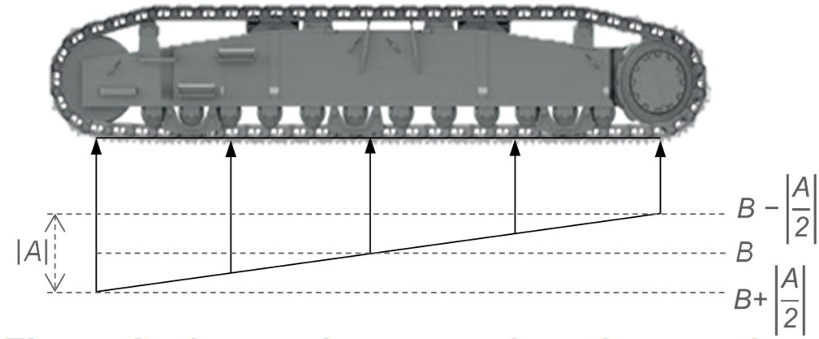
\includegraphics[width=\linewidth]{fig_08}
\caption{ Aperçu des expressions des pressions 
minimale, maximale et moyenne. \label{Cy_11_Ch_01_TD_01_fig_08}}
\end{marginfigure}
La figure \ref{Cy_11_Ch_01_TD_01_fig_08} permet de remarquer que $B$ 
(respectivement $D$), toujours positive, est la 
pression moyenne de la répartition 
trapézoïdale gauche (respectivement droite) 
et que $A$ (respectivement $C$), positive ou 
négative, en est l’écart entre sa pression 
avant et arrière. Ainsi, la pression maximale 
du sol sur la chenille gauche vaut toujours 
$B+\left|\dfrac{A}{2}\right|$ (respectivement  $D+\left|\dfrac{C}{2}\right|$ à droite).

Ainsi, pour estimer la pression maximale exercée au sol, l’ordinateur de bord estime d’abord la 
position de $E$ et la valeur de $\indice{F}{eq}$ en fonction des données renvoyées à tout instant par les capteurs 
présents sur les différents axes de la foreuse. Ensuite, il détermine les valeurs des pressions $A$, $B$, 
$C$ et $D$ grâce aux équations précédentes avec \textbf{l’hypothèse assez réaliste où $C = A$} et en déduit la 
pression maximale. Enfin, il renvoie à l’écran la visualisation << aplatie >> des distributions de pression 
et sonne l’alarme en cas d’approche de la pression maximale autorisée rentrée par l’utilisateur. 

\question{Après avoir précisé l’expression des paramètres $A$, $B$, $C$ et $D$, donner l’expression de la pression maximale de chacune des répartitions estimées (gauche et droite) en fonction des données connues par la machine ($L$, $l$, $a$, $e$, $\theta$ et $\indice{F}{eq}$ uniquement). }

\question{En déduire que l’expression unique de la pression maximale sous la foreuse s’écrit : $\indice{p}{max}=\dfrac{-\indice{F}{eq}}{2Ll}\left(1+ \dfrac{e|\cos\theta|}{a}+ \dfrac{6e|\sin\theta|}{L}\right)$.}
